\documentclass[a4paper]{article}

\usepackage[english]{babel}
\usepackage[utf8]{inputenc}
\usepackage{amsmath}
\usepackage{graphicx}
%\usepackage{yhmath}
\usepackage{amsmath,amsthm,amssymb}
\newtheorem{thm}{Theorem}
\newcount\colveccount
\newcommand*\colvec[1]{
        \global\colveccount#1
        \begin{pmatrix}
        \colvecnext
}
\def\colvecnext#1{
        #1
        \global\advance\colveccount-1
        \ifnum\colveccount>0
                \\
                \expandafter\colvecnext
        \else
                \end{pmatrix}
        \fi
}
\begin{document}

\title{Vector Project}

\author{Ananya Cleetus}

\date{\today}



\maketitle

\section{Converting Latitude and Longitude to Cartesian Coordinates }

To convert from latitude and longitude to Cartesian coordinates, first convert the longitude and latitude to radians. 
\bigskip
\begin{center}
\textbf{Latitude (in radians) is Latitude (in decimal degrees) *$\frac{\pi}{180}$}\\
\textbf{Longitude (in radians) is Longitude (in decimal degrees) *$\frac{\pi} {180}$}\\
\end{center}
\bigskip
Since the $z$-coordinate of Cartesian coordinates goes in the direction of the poles, to find the $z$-coordinate, simply multiply the radius of the Earth by the sine of the latitude in radians. This is because given a triangle using the latitude as the angle measure, the side of the triangle being the radius of the Earth, $r$, would need to be multiplied by the sine of the angle to yield the change or height in the $x$-direction.

\begin{center}
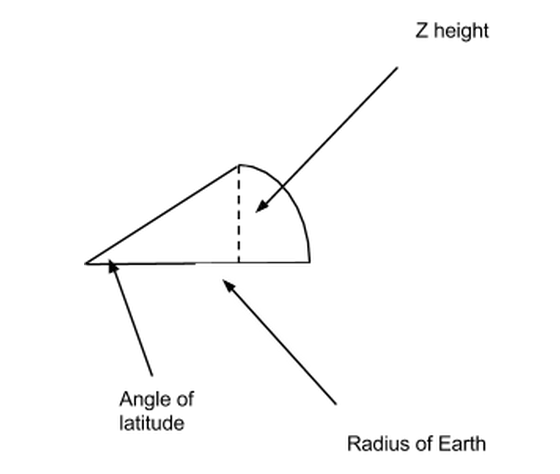
\includegraphics[scale=.375]{vec1.png}
\end{center}

For the $y$-coordinate of Cartesian coordinates, it’s harder to draw a diagram but essentially multiply the Earth’s radius $r$ by the sine of the longitude and the cosine of the latitude. For the $x$-coordinate, this is a bit different, and one would need to multiply the Earth’s radius $r$ by the cosine of the latitude and the cosine of the longitude. This works since the latitude and longitude are based in angle range as they move away from the Equator or Prime Meridian, respectively. The formulas are:

\begin{center}
\textbf{$x = cos($latitude$) * cos($longitude$) * r $}\\
\textbf{$y = cos($latitude$) * sin($longitude$) * r $ }\\
\textbf{$z = sin($latitude$) * r $ }\\
\end{center}

So latitude $a$, longitude $b$ = $\colvec{3}{rcos(a)cos(b)}{rcos(a)sin(b)}{ rsin(a)}$

\begin{center}
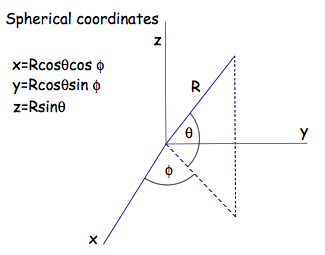
\includegraphics[scale=.375]{vec2.png}
\end{center}
\section{Finding the Distance Between Two Points on the Earth’s Surface}

If $d$ is the Euclidean (straight-line) distance between any two points on the Earth's surface, $d$ in terms of the position vectors of the two points is found using the Pythagorean theorem: 

\begin{center}
\textbf{$d^{2} = (x_{2} - x_{1})^{2} + (y_{2} - y_{1})^{2} + (z_{2} - z_{1})^{2}$}
\end{center}

In order to find the arc length $D$, the angle $\theta$ and Euclidean distance $d$ need to be calculated. For the triangle portion of the sector, which has Euclidean distance $d$, the angle of the sector $\theta$ is related such that the $sine$ of half the sector angle is equal to the half the Euclidean distance $d$ over the radius, $r$. Visually, this is done by dividing the sector triangle into two equal halves with a perpendicular bisector such that both triangles have a leg $\dfrac{d}{2}$ and hypotenuse $r$. Mathematically, this can be expressed as follows: 


\begin{center}
\textbf{$sin\left(\dfrac{\theta}{2	}\right) = \dfrac{\dfrac{d}{2}}{r}$}\\
\medskip
\textbf{$sin\left(\dfrac{\theta}{2	}\right) = \dfrac{d}{2r}$}\\
\end{center}

For the entire sector, however, the angle is $\theta$. The relationship between $sin(\theta)$ and $sin\left(\dfrac{\theta}{2}\right)$ can be found using the double angle identify for $sin(2\phi)$ for which $\phi$ would be equal to $\dfrac{\theta}{2}$.

\begin{center}
\textbf{$sin(2\phi) = 2sin(\phi)*cos(\phi)$}\\
\medskip
\textbf{$\phi = \dfrac{\theta}{2}$}\\
\medskip
\textbf{$sin(2\left(\dfrac{\theta}{2}\right)) = 2sin(\left(\dfrac{\theta}{2}\right))*cos(\left(\dfrac{\theta}{2}\right))$}\\
\end{center}

Since the relationship is defined for $sin\left(\dfrac{\theta}{2	}\right)$, I can simplify the part of the double angle identity with $cos\left(\dfrac{\theta}{2	}\right)$ to an equivalent form in terms of $sine$ using a trigonometric identity:

\begin{center}
\textbf{$sin^2\left(\dfrac{\theta}{2}\right) + cos^2\left(\dfrac{\theta}{2	}\right) = 1$}\\
\medskip
\textbf{$cos^2\left(\dfrac{\theta}{2	}\right) = 1-sin^2\left(\dfrac{\theta}{2}\right)$}\\
\medskip
\textbf{$cos\left(\dfrac{\theta}{2	}\right) = \sqrt{1-sin^2\left(\dfrac{\theta}{2}\right)}$}\\
\end{center}

Substituting the value of $cos\left(\dfrac{\theta}{2	}\right)$ back into the previous equation: 

\begin{center}
\textbf{$sin(2\left(\dfrac{\theta}{2}\right)) = 2sin(\left(\dfrac{\theta}{2}\right))*\sqrt{1-sin^2\left(\dfrac{\theta}{2}\right)}$}\\
\medskip
\textbf{$sin(\theta) = 2sin(\left(\dfrac{\theta}{2}\right))*\sqrt{1-sin^2\left(\dfrac{\theta}{2}\right)}$}\\
\end{center}

Now that the $sine$ of the sector angle $\theta$ is in terms of the previously defined $sin(\left(\dfrac{\theta}{2}\right))$, this can be replaced with $\dfrac{d}{2r}$ as previously found by using the sector triangle: 

\begin{center}
\textbf{$sin(\theta) = 2sin(\left(\dfrac{\theta}{2}\right))*\sqrt{1-sin^2\left(\dfrac{\theta}{2}\right)}$}\\
\medskip
\textbf{$sin\left(\dfrac{\theta}{2}\right) = \dfrac{d}{2r}$}\\
\medskip
\textbf{$sin(\theta) = 2\left(\dfrac{d}{2r}\right)*\sqrt{1-\left(\dfrac{d}{2r}\right)^2}$}\\
\medskip
\textbf{$sin(\theta) = \left(\dfrac{d}{r}\right)*\sqrt{1-\left(\dfrac{d^2}{(2r)^2}\right)}$}\\
\medskip
\textbf{$sin(\theta) = \dfrac{d}{r}*\sqrt{1-\left(\dfrac{d^2}{4r^2}\right)}$}\\
\medskip
\textbf{$sin(\theta) = \dfrac{d}{r}*\sqrt{\left(\dfrac{4r^2}{4r^2}\right)-\left(\dfrac{d^2}{4r^2}\right)}$}\\
\medskip
\textbf{$sin(\theta) = \dfrac{d}{r}* \sqrt{\dfrac{4r^2-d^2}{4r^2}}$}\\
\medskip
\textbf{$sin(\theta) = \dfrac{d}{r}* \dfrac{\sqrt{4r^2-d^2}}{2r}$}\\
\medskip
\textbf{$sin(\theta) = \dfrac{d}{2r^2}* \sqrt{4r^2-d^2}$}\\
\medskip
\textbf{$sin(\theta) = \dfrac{d\sqrt{4r^2-d^2}}{2r^2}$}\\
\end{center}

With $sin(\theta)$ expressed as a relation between the radius and Euclidean distance, the arc length $l$ can be found using the formula for arc length, given a radius and angle: 

\begin{center}
\textbf{$l = r * \theta$}\\
\textbf{$l = r * sin^{-1}(sin(\theta))$}\\
\medskip
\textbf{$sin(\theta) = \dfrac{d\sqrt{4r^2-d^2}}{2r^2}$}\\
\medskip
\textbf{$l = r * sin^{-1}\left(\dfrac{d\sqrt{4r^2-d^2}}{2r^2}\right)$}\\
\end{center}
The arc length $l$ is finally in terms of the radius and Euclidean distance. The Euclidean distance $d$ can be found from the position vectors: 

\begin{center}
\textbf{$d^{2} = (x_{2} - x_{1})^{2} + (y_{2} - y_{1})^{2} + (z_{2} - z_{1})^{2}$}
\end{center}

The Euclidean distance can also be derived from the longitude and latitude. For two points (assuming the latitude and longitude are in radians*):
\begin{center}
\textbf{Point a:}\\
\textbf{latitude = $lat_{1}$}\\
\textbf{longitude = $lon_{1}$}\\
\medskip
\textbf{Point b:}\\
\textbf{latitude = $lat_{2}$}\\
\textbf{longitude = $lon_{2}$}\\
\medskip
\textbf{$x = cos($latitude$) * cos($longitude$) * r $}\\
\textbf{$y = cos($latitude$) * sin($longitude$) * r $ }\\
\textbf{$z = sin($latitude$) * r $ }\\
\medskip
\textbf{$x_1 = cos(lat_1) * cos(lon_1) * r $}\\
\textbf{$y_1 = cos(lat_1) * sin(lon_1) * r $ }\\
\textbf{$z_1 = sin(lat_1) * r $ }\\
\medskip
\textbf{$x_2 = cos(lat_2) * cos(lon_2) * r $}\\
\textbf{$y_2 = cos(lat_2) * sin(lon_2) * r $ }\\
\textbf{$z_2 = sin(lat_2) * r $ }\\
\medskip
\textbf{$a = \colvec{3}{x_{1}}{y_{1}}{z_{1}}$}\\
\medskip
\textbf{$b=\colvec{3}{x_{2}}{y_{2}}{z_{2}}$}\\
\medskip
\textbf{$a = \colvec{3}{rcos(lat_1)cos(lon_1)}{rcos(lat_1)sin(lon_1)}{rsin(lat_1) }$}\\
\medskip
\textbf{$b = \colvec{3}{rcos(lat_2)cos(lon_2)}{rcos(lat_2)sin(lon_2)}{rsin(lat_2) }$}\\
\medskip
\textbf{$d^{2} = (rcos(lat_2)cos(lon_2)-rcos(lat_1)cos(lon_1))^{2} + (rcos(lat_2)sin(lon_2)-rcos(lat_1)sin(lon_1))^{2} + (rsin(lat_2) -rsin(lat_1))^{2}$}
\medskip
\end{center}
\textit{*Latitude (in radians) is Latitude (in decimal degrees) *$\frac{\pi}{180}$\\
Longitude (in radians) is Longitude (in decimal degrees) *$\frac{\pi} {180}$\\
}
\section{Finding the Distance Between My House and My Grandmother's House}
Using the formula for the arc length: 
\begin{center}
\textbf{$l = r * sin^{-1}\left(\dfrac{d\sqrt{4r^2-d^2}}{2r^2}\right)$}\\
\end{center}
And the formula for finding the Euclidean distance from the longitude and latitude of two points: 
\begin{center}
\textbf{$d^{2} = (rcos(lat_2)cos(lon_2)-rcos(lat_1)cos(lon_1))^{2} + (rcos(lat_2)sin(lon_2)-rcos(lat_1)sin(lon_1))^{2} + (rsin(lat_2) -rsin(lat_1))^{2}$}
\end{center}

I can find out the distance from my house to my grandmother's. My house is located in Pittsburgh, PA, in the United States. Its latitude and longitude are 40.3127878 and -80.0792457, respectively. My grandmother's house is located in Greater Kailash Colony, New Delhi, India. Its latitude and longitude are 28.5523666 and 77.2429581, respectively. 
\\\\
First, I converted the longitude and latitude in degrees to that in radians by multiplying by $\dfrac{\pi}{180}$. 

\begin{center}
\textbf{My House (Point 1):}\\ 
\medskip
\textbf{Latitude (in radians) $= 40.3127878 * \dfrac{\pi}{180} = 0.70359087777$}\\
\medskip
\textbf{Longitude (in radians) $= -80.0792457 * \dfrac{\pi}{180}= -1.3976465$}\\ 
\medskip
\textbf{My Grandmother's House (Point 2):}\\
\bigskip
\textbf{Latitude (in radians)$ = 28.5523666 * \dfrac{\pi}{180}=0.49833280641$}\\
\medskip
\textbf{Longitude (in radians)$ = 77.2429581 * \dfrac{\pi}{180}=1.3481439428$}\\ 
\end{center}

Then, I put the radian values of latitude and longitude in the Euclidean distance formula, using 6371 km as $r$, the Earth's radius:

\begin{center}
\textbf{$d^{2} = ((6371)cos(0.49833280641)cos(1.3481439428)-(6371)cos(0.70359087777)cos(-1.3976465))^{2} + ((6371)cos(0.49833280641)sin(1.3481439428)-(6371)cos(0.70359087777)sin(-1.3976465))^{2} + ((6371)sin(0.49833280641) -(6371)sin(0.70359087777))^{2}$}\\
\medskip
\textbf{$d^2 \approx (1305.56-884.27)^2 + (5458.02-(-5055.8))^2 +(3217.16-4354.69)^2 $}\\
\medskip
\textbf{$d^2 \approx (421.29)^2 + (10513.82)^2 + (-1137.53)^2$}\\
\medskip
\textbf{$d \approx 10583.57  $ km}
\end{center}

With the calculated Euclidean distance and radius of 6371 km, I can now solve for the surface distance/arc length $l$: 

\begin{center}
\textbf{$l \approx r * sin^{-1}\left(\dfrac{d\sqrt{4r^2-d^2}}{2r^2}\right)$}\\
\medskip
\textbf{$l \approx (6371) * sin^{-1}\left(\dfrac{(10583.57)\sqrt{4(6371)^2-(10583.57)^2}}{2(6371)^2}\right)$}\\
\medskip
\textbf{$l \approx (6371) * sin^{-1}\left(\dfrac{(10583.57)\sqrt{(162358564)-(112011953.9)}}{81179282}\right)$}\\
\medskip
\textbf{$l \approx (6371) * sin^{-1}\left(\dfrac{(10583.57)\sqrt{50346610.1}}{81179282}\right)$}\\
\medskip
\textbf{$l \approx (6371) * sin^{-1}\left(\dfrac{(10583.57)(7095.53)}{81179282}\right)$}\\
\medskip
\textbf{$l \approx (6371) * sin^{-1}(.9250640877)$}\\
\medskip
\textbf{$l \approx 7525.45$ km}\\
\medskip
\end{center}
\end{document}
